\chapter{Final Phase}
\label{chap:FinalPhase}

The product prototype was finished during Sprint 4. A functional website and mobile app containing most of the functionality previously specified. In this final phase of the project, the main goal was to finish the project report, test the prototype and fix any bugs that were found.

\section{Phase Plan}
\label{sec:FinalPlan}

During the final phase the product prototypes mainly went through testing and bug fixing. The main focus of this phase was, however, completing the report of the project and preparing for the presentation. This final sprint started with each person uploading their work to the shared drive, followed by each member proofreading, editing and correcting the work before the final version was implemented in LaTeX. Other tools, like the work sheets and YouTrack, had their finishing updates.

\paragraph{} The team members responsible for the report did the main proofreading, editing, and correction. Each person responsible for sections that were unfinished had to finish their sections and upload their work so that the group could finish the report. Another focus was to prepare for the presentation, to be held November 20th, 2014. The main tasks of preparation included creating slides and rehearsing for the presentation.

\paragraph{} The development team was reduced to only one person who was responsible for setting up the website to \href{www.mysplot.com}{http://www.mysplot.com} and the app to Google Play, bug fixing, and final touches where necessary. Each member of the team had to execute a set of test cases and report the results to ensure that the product was ready for delivery. The test cases can be found in appendix \ref{chap:TestingTPlan}.
The tasks to be finished are mentioned in detail in the backlog for this phase.

\section{Workload and Duration}
\label{sec:FinalWorkload}
%
\begin{minipage}{\linewidth}
\centering
\setlength{\tabcolsep}{22pt}
\textbf{Final Phase:} 
\smallskip
\rowcolors{1}{blue!20}{blue!10}
\begin{tabular}{ |l l| }
	\hline
	\it{Duration} & 2 weeks \\
	\it{Start} & November 3rd. \\
	\it{End} & November 16th. \\
	\it{Workload} & Hours spent by the entire group on Sprint 2. \\
	\it{Goal} & 40 - 50 hours per person \\
	\hline
\end{tabular}
\end{minipage}
\bigskip
%
\begin{minipage}{\linewidth}
\setlength{\tabcolsep}{25pt}
\centering
\rowcolors{1}{blue!20}{blue!10}
\begin{tabular}{ |l|l| }
	\hline
	\multicolumn{2}{|c|}{\cellcolor{gray!25} Workload} \\
	\hline
	\it{Planning} & 60 hrs \\
	\it{Development} & 5 hrs \\
	\it{Design} & None \\
	\it{Documentation} & 237 hrs \\
	\it{Testing \& Bug Fixing} & 19 hrs \\
	\hline
	\it{Total workload} & 327 hrs \\
	\hline
\end{tabular}
\captionof{table}{\label{tab:FinalWorkload} Workload of Final Phase} 
\end{minipage}

\section{Phase Backlog}
\label{sec:FinalBacklog}

Below is a table depicting the sprint backlog for the final phase. The estimated and actual time are also displayed.

\begin{minipage}{\linewidth}
\setlength{\tabcolsep}{12pt}
\centering
\rowcolors{1}{blue!20}{blue!10}
\begin{tabular}{|p{1cm}|p{4cm}|p{2cm}|p{2cm}|}
\hline
\cellcolor{gray!25} ID & \cellcolor{gray!25} Description & \cellcolor{gray!25} Estimated Time & \cellcolor{gray!25} Actual Time \\
\hline
RPT-8 & \it{Further Work completion} & 30 hours & 41 hours\\
RPT-15 & \it{Appendices completion} & 15 hours & ? \\
RPT-18 & \it{Test Cases and Test Results} &  2 hours & 4 hours \\
RPT-19 & \it{Testing and Documentation} & 15 hours & ? \\
RPT-42 & \it{Sprint 3 completion} & 15 hours & ? \\
RPT-43 & \it{Sprint 4 completion} & 15 hours & ? \\
RPT-44 & \it{Final Phase completion} & 15 hours & ? \\
RPT-76 & \it{Architecture completion} & 15 hours & ? \\
RPT-78 & \it{LaTeX Implementation} &  & ? \\
RPT-79 & \it{Slide presentation} & 15 hours & ? \\
\hline
\end{tabular}
\captionof{table}{Backlog for the final phase.} 
\end{minipage}

\subsection{Completing the report}
\label{sec:FinalReport}

To keep track of which chapters for the report are incomplete the team used a customized Google Document including all chapters which are marked differently based on status. The document utilized color coding to represent the status of the chapters, as illustrated in figures \ref{fig:FinalColors} and \ref{fig:FinalReportBacklog}.

\begin{figure}[ht!]
\centering
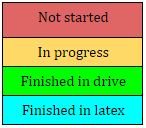
\includegraphics[width=90mm]{./FinalSprint/img/Colors.png}
\caption{Colors used in for the Sprint report backlog. \label{fig:FinalColors}}
\end{figure}

\begin{figure}[ht!]
\centering
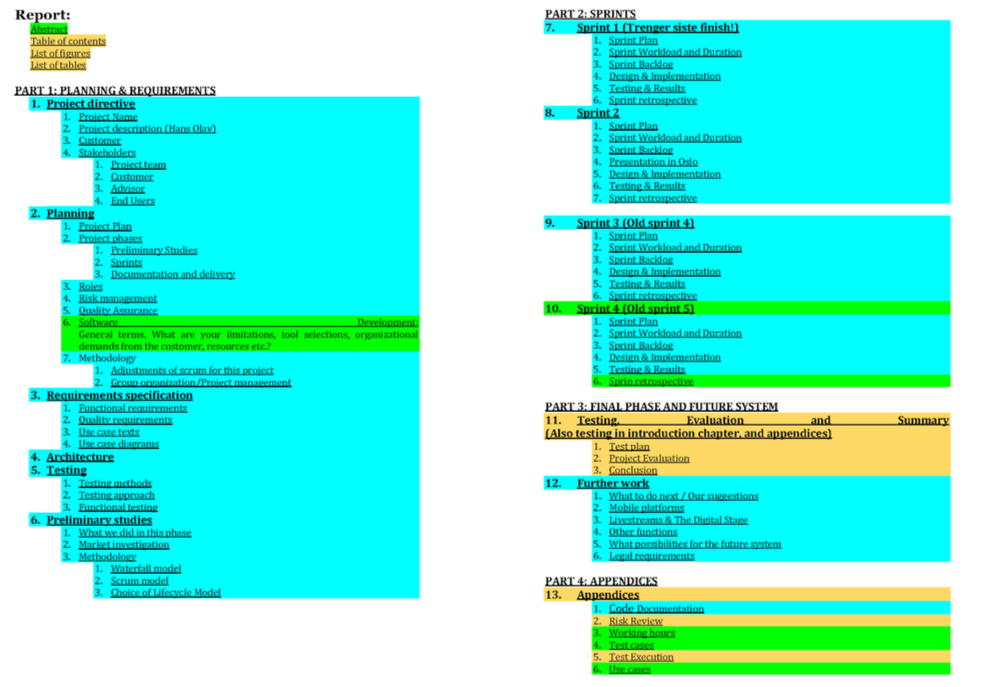
\includegraphics[width=90mm]{./FinalSprint/img/ReportBacklog.png}
\caption{A remade Sprint Report Backlog, made for quickly keeping status of the report development. \label{fig:FinalReportBacklog}}
\end{figure}

\section{Testing}
\label{sec:FinalTesting}

During the final phase of the project, the product was thoroughly tested by the whole group. Both through a complete system test using the test cases detailed in Appendix~\ref{chap:TestingTPlan}, and through general usage of the website and app in over a week. That way a few remaining bugs were discovered before being fixed by the lead developer. The system test was a functional test, executed to ensure the group that all functionality was working as expected. Table \ref{tab:FinalTestingBugs} contains a list of the bugs that were fixed.

\rowcolors{1}{blue!20}{blue!10}
\begin{tabular}{|p{0.2\linewidth} p{0.8\linewidth}|}
\hline
\cellcolor{gray!25} \textbf{Bug ID} & \cellcolor{gray!25} \textbf{Description} \\
\hline
\multicolumn{2}{|c|}{\cellcolor{gray!25} Website} \\
1 & Favicon was not correctly updated. \\
2 & Save all images with JPG extension instead of JPG \& JPEG \\
3 & Disallow numbers in first/last names. Allow dashes. Force password to be at least 6 chars long. \\
4 & Disallow events to be hosted in the past or more than 1 year into the future. \\
5 & Infinite scroll stopped working due to changes with autocomplete address search. \\
6 & All locations were mapped into north-eastern hemisphere. \\
7 & Search content boxes were of different sizes. \\
\multicolumn{2}{|c|}{\cellcolor{gray!25} Application} \\
8 & Some devices were unable to "OK" the taken picture.
\end{tabular}
\captionof{table}{Table showing bugs fixed during the final phase. \label{tab:FinalTestingBugs}}
%\medskip
%Website: 
%\begin{description}
%  \item[Bug 1] \hfill \\
%  Favicon was not correctly updated.
%  \item[Bug 2] \hfill \\
%  Save all images with JPG extension instead of JPG \& JPEG.
%  \item[Bug 3] \hfill \\
%  Disallow numbers in first/last names. Allow dashes. Force password to be at least 6 chars long.
%  \item[Bug 4] \hfill \\
%  Disallow events to be hosted in the past or more than 1 year into the future.
%  \item[Bug 5] \hfill \\
%  Infinite scroll stopped working due to changes with autocomplete address search.
%  \item[Bug 6] \hfill \\
%  All locations were mapped into north-eastern hemisphere
%  \item[Bug 7] \hfill \\
%  Search content boxes were of different sizes.
%\end{description}
%\medskip
%App: 
%\begin{description}
%  \item[Bug 8] \hfill \\
%  Some devices were unable to "OK" the taken picture.
%\end{description}
%
\begin{minipage}{\linewidth}
\setlength{\tabcolsep}{15pt}
\centering
\rowcolors{1}{blue!20}{blue!10}
\begin{tabular}{ |l|p{70mm}| }
	\hline
	\multicolumn{2}{|c|}{\cellcolor{gray!25} \textbf{Preview of Test Case 1}} \\
	\hline
	\it{\cellcolor{gray!25}Item} & {\cellcolor{gray!25} Description } \\
	\hline
	\it{\cellcolor{gray!25}Test Name } & Create User on the Web Page \\ \hline
	\it{\cellcolor{gray!25}Test ID} & TC1 \\ \hline
	\it{\cellcolor{gray!25}Feature to be tested} & Creating a new unique user profile \\ \hline
	\it{\cellcolor{gray!25}Requirements} & F1  \\ \hline
	\it{\cellcolor{gray!25}Pre-conditions} & User must have a supported web browser  \\ \hline
	\it{\cellcolor{gray!25}Steps of Execution} & Open a browser. Enter www.mysplot.com. Click the ``Sign up'' button in the upper right hand corner. Fill in first name, last name, a desired username and password in their respective fields, choose gender and finally click Sign Up. \\ \hline
	\it{\cellcolor{gray!25}Expected results} & An error message will be displayed if fields are incorrect or taken. If all information input is valid, a user will be created on the website and saved in the database.  \\
	\hline
\end{tabular}
\captionof{table}{Preview of Test case 1}
\medskip
\end{minipage}
%
\begin{minipage}{\linewidth}
\setlength{\tabcolsep}{15pt}
\centering
\rowcolors{1}{blue!20}{blue!10}
\begin{tabular}{ |l|p{70mm}| }
	\hline
	\multicolumn{2}{|c|}{\cellcolor{gray!25} \textbf{Preview of Test Results, Yngve}} \\
	\hline
	\it{\cellcolor{gray!25}Test Case ID} & {\cellcolor{gray!25} Results } \\
	\hline
	\it{\cellcolor{gray!25}TC1} & \begin{enumerate}[label=\alph*)]
	                                \item As expected, error message
	                                \item as expected
	                              \end{enumerate}\\ \hline
	\it{\cellcolor{gray!25}TC2} & \begin{enumerate}[label=\alph*)]
	                                \item As expected
	                                \item As expected	
	                              \end{enumerate}\\ \hline
	\it{\cellcolor{gray!25}TC3} & Was signed out \\ \hline
	\it{\cellcolor{gray!25}TC4} & As expected \\ \hline
	\it{\cellcolor{gray!25}TC5} & As expected \\ \hline
	\it{\cellcolor{gray!25}TC6} & As expected, got photo \\ \hline
\end{tabular}
\captionof{table}{Preview of Test Results by Yngve}
\medskip
\end{minipage}

\section{Results}
\label{sec:FinalResults}

The product prototype was practically finished in the previous sprint, and each member tested the final version of the product from the user perspective, reporting bugs and issues, which were actively corrected as they were reported. This detection and fixing of bugs ensured a stable and well-functioning version of the website and app would be ready for delivery. 

\paragraph{} For the project reflection, each member had to supply their experiences with the entire project. With this reflection, the group learned about the challenges and progress the members of the group had faced and achieved individually and together. 

\paragraph{} The major result of the sprint was finishing the report. During the sprint each member involved in the report had to ensure that every section they were responsible for was completed. The parts that were finished finished are specified further in the Phase Plan. Proofreading, editing, and correction of grammar and spelling errors all contributed to improving every section of the report. Finally, the report was implemented in LaTeX giving it a professional touch. This was time consuming, but improved the layout and readability of the report.

\paragraph{} The concluding tasks of the sprint was preparation for the presentation to be held for both the customer and the examiner. This is an ongoing task. Hopefully the slides, demo, and presentation will go as planned and well.


\section{Sprint Retrospective}
\label{sec:FinalRetrospective}

\subsection{Start Doing}
\begin{itemize}
\item Project Reflection
\item Prepare presentation
\item Print report
\end{itemize}

\subsection{Stop Doing}
\begin{itemize}
\item Taking too long breaks during work
\item Sleeping way into the day
\item Being ineffective in the mornings
\end{itemize}

\subsection{Continue Doing}
\begin{itemize}
\item Working effectively when in the flow.
\item Proofreading
\item LaTeX implementation
\item Taking awesome notes during meetings. 
\end{itemize}

\section{Group Dynamics}
\label{sec:FinalDynamics}
Over the course of the entire project the team has made substantial progress in working together. This is evident in the way the work process has changed and improved each sprint. Every member has given their best and spent as much time on the project as they could manage. Upon finishing this last sprint all members of the team are proud of the product, the report, and their work efforts realized as part of the project. As well as the progress and experience they made in working as a team and group dynamics, and acquiring new knowledge and skills. In this last phase the entire group greatly contributed to finishing a working product and an extensive report describing every aspect of the project, in a smooth work flow that is far superior to our first weeks of working together. 
